%
% Template Laporan Skripsi/Thesis 
%
% @author  Andreas Febrian, Lia Sadita 
% @version 1.03
%
% Dokumen ini dibuat berdasarkan standar IEEE dalam membuat class untuk 
% LaTeX dan konfigurasi LaTeX yang digunakan Fahrurrozi Rahman ketika 
% membuat laporan skripsi. Konfigurasi yang lama telah disesuaikan dengan 
% aturan penulisan thesis yang dikeluarkan UI pada tahun 2008.
%

%
% Tipe dokumen adalah report dengan satu kolom. 
%
\documentclass[12pt, a4paper, onecolumn, oneside, final]{report}

% Load konfigurasi LaTeX untuk tipe laporan thesis
\usepackage{_internals/uithesis}
\usepackage{_internals/tikz-uml}

% Daftar pemenggalan suku kata dan istilah dalam LaTeX
\input{_internals/hype.indonesia}

% Load konfigurasi khusus untuk laporan yang sedang dibuat
%-----------------------------------------------------------------------------%
% Informasi Mengenai Dokumen
%-----------------------------------------------------------------------------%
% 
% Judul laporan. 
\var{\judul}{Implementasi Augmentasi Data Berbasis Variational Autoencoder untuk Klasifikasi Autism Spectrum Disorder Menggunakan Sinyal EEG}
% 
% Tulis kembali judul laporan, kali ini akan diubah menjadi huruf kapital
\Var{\Judul}{\MakeUppercase{\judul}}
% 
% Tulis kembali judul laporan namun dengan bahasa Ingris
\var{\judulInggris}{Analysis of Data Augmentation Using Variational Autoencoder for EEG-Based Autism Spectrum Disorder Classification}

% Tulis kembali judul laporan dengan bahasa Ingris, kali ini akan diubah menjadi huruf kapital
\var{\JudulInggris}{\MakeUppercase{\judulInggris}}

% 
% Tipe laporan, dapat berisi Skripsi, Tugas Akhir, Thesis, atau Disertasi
\var{\type}{Skripsi}
% 
% Tulis kembali tipe laporan, kali ini akan diubah menjadi huruf kapital
\Var{\Type}{\MakeUppercase{\type}}
% 
% Tulis nama penulis 
\var{\penulis}{Wendy Dharmawan}
% 
% Tulis kembali nama penulis, kali ini akan diubah menjadi huruf kapital
\Var{\Penulis}{\MakeUppercase{\penulis}}

% 
% Tulis NPM penulis
\var{\npm}{2206059591}
% 
% Tuliskan Fakultas dimana penulis berada
\var{\fakultas}{Teknik}
\Var{\Fakultas}{\MakeUppercase{\fakultas}}
% 
% Tuliskan Program Studi yang diambil penulis
\var{\program}{S1 Teknik Komputer}
\Var{\Program}{\MakeUppercase{\program}}
% 
% Tuliskan tahun publikasi laporan
\Var{\bulan}{Juni}
\Var{\tahun}{2026}
% 
% Tuliskan gelar yang akan diperoleh dengan menyerahkan laporan ini
\var{\gelar}{Sarjana Teknik}
% 
% Tuliskan tanggal pengesahan laporan, waktu dimana laporan diserahkan ke 
% penguji/sekretariat
\var{\tanggalPengesahan}{2 Juni 2026} 
% 
% Tuliskan tanggal keputusan sidang dikeluarkan dan penulis dinyatakan 
% lulus/tidak lulus
\var{\tanggalLulus}{ Agustus 2026}
% 
% Tuliskan pembimbing 
\var{\pembimbing}{Dr. Prima Dewi Purnamasari, S.T., M.Sc.}
\var{\kadept}{Dr. Muhammad Salman, ST., M.IT.}
\var{\kaprodi}{Dr. Prima Dewi Purnamasari, S.T., M.Sc.}
\var{\pa}{Prof. Dr.-Ing. Kalamullah Ramli}
\var{\pengujisatu}{Dr. Eng. Mia Rizkinia, S.T, M.T.}
\var{\pengujidua}{Prof. Dr. Ir. Anak Agung Putri Ratna, M.Eng}
% 
% Alias untuk memudahkan alur penulisan paa saat menulis laporan
\var{\saya}{Penulis}

%-----------------------------------------------------------------------------%
% Judul Setiap Bab
%-----------------------------------------------------------------------------%
% 
% Berikut ada judul-judul setiap bab. 
% Silahkan diubah sesuai dengan kebutuhan. 
% 
\Var{\kataPengantar}{Kata Pengantar}
\Var{\babSatu}{Pendahuluan}
\Var{\babDua}{Tinjauan Pustaka}
\Var{\babTiga}{Perancangan dan Implementasi Sistem}
\Var{\babEmpat}{Eksperimen dan Analisis}
\Var{\babLima}{Penutup}

% Daftar istilah yang mungkin perlu ditandai 

\begin{longtable}{p{3cm} p{11cm}}

\textbf{Alpha} & Pita frekuensi alpha: komponen gelombang EEG pada rentang 8--13\,Hz yang dominan pada wilayah oksipital saat kondisi rileks dengan mata tertutup. \\

\textbf{Artefak} & Komponen sinyal non-neural pada rekaman EEG yang berasal dari aktivitas fisiologis (kedipan mata, gerakan otot) maupun gangguan eksternal seperti interferensi perangkat elektronik. \\

\textbf{Augmentasi} & Augmentasi data (\textit{data augmentation}): teknik penambahan variasi data pelatihan secara artifisial untuk meningkatkan performa model dan mengurangi \textit{overfitting}. \\

\textbf{ASD} & Autism Spectrum Disorder: gangguan perkembangan saraf yang ditandai hambatan komunikasi, interaksi sosial, serta perilaku repetitif. \\

\textbf{Beta} & Pita frekuensi beta: komponen EEG pada rentang 13--30\,Hz yang berkaitan dengan aktivitas kognitif aktif, konsentrasi, dan pemecahan masalah. \\

\textbf{Decoder} & Komponen model generatif yang memetakan variabel laten untuk merekonstruksi sinyal EEG sintetis. \\

\textbf{Delta} & Pita frekuensi delta: rentang 0.5--4\,Hz yang dominan pada kondisi tidur nyenyak dan proses pemulihan fisiologis. \\

\textbf{DNN} & Deep Neural Network: jaringan saraf tiruan dalam dengan beberapa hidden layer untuk mempelajari pola kompleks. \\

\textbf{EEG} & Electroencephalography: metode perekaman aktivitas listrik otak secara non-invasif menggunakan elektroda pada kulit kepala. \\

\textbf{ELBO} & Evidence Lower Bound: fungsi objektif pada VAE yang terdiri dari reconstruction loss dan KL divergence. \\

\textbf{Encoder} & Encoder: komponen model yang memetakan data input ke ruang laten berdimensi rendah berbasis distribusi probabilistik. \\

\textbf{FFT} & Fast Fourier Transform: metode transformasi sinyal dari domain waktu ke domain frekuensi. \\

\textbf{FID} & Fréchet Inception Distance: metrik untuk mengukur kesamaan distribusi antara data asli dan data sintetis. \\

\textbf{Gamma} & Pita frekuensi gamma: sinyal EEG dengan frekuensi $>30\,Hz$ yang terkait proses kognitif tingkat tinggi. \\

\textbf{Generalisasi} & Kemampuan model mempertahankan performa pada data yang tidak terlihat selama pelatihan. \\

\textbf{Hyperparameter} & Parameter yang ditentukan sebelum pelatihan seperti learning rate atau jumlah estimators. \\

\textbf{ICA} & Independent Component Analysis: metode pemisahan sumber sinyal untuk mengurangi artefak EEG. \\

\textbf{KL} & Kullback--Leibler Divergence: regularisasi pada VAE untuk menjaga distribusi laten mendekati distribusi normal. \\

\textbf{Latent} & Latent Space: ruang representasi berdimensi rendah yang menangkap struktur penting data. \\

\textbf{mRMR} & Minimum Redundancy Maximum Relevance: metode seleksi fitur berbasis relevansi maksimum dan redundansi minimum. \\

\textbf{Overfitting} & Kondisi ketika model terlalu menyesuaikan data pelatihan sehingga menurunkan performa pada data baru. \\

\textbf{PSD} & Power Spectral Density: distribusi energi sinyal terhadap frekuensi. \\

\textbf{Preprocessing} & Pra-pemrosesan: tahap persiapan data EEG seperti filtering, normalisasi, dan segmentasi. \\

\textbf{SWD} & Sliced Wasserstein Distance: metrik untuk mengukur kesamaan distribusi data melalui proyeksi satu dimensi. \\

\textbf{Theta} & Pita frekuensi theta: rentang 4--8\,Hz yang terkait memori dan kondisi mengantuk. \\

\textbf{U-shaped} & U-shaped spectral profile: pola spektral dengan peningkatan daya pada frekuensi rendah dan tinggi serta penurunan pada frekuensi menengah. \\

\textbf{VAE} & Variational Autoencoder: model generatif berbasis encoder-decoder untuk mempelajari ruang laten probabilistik. \\

\textbf{XGBoost} & Extreme Gradient Boosting: algoritma ensemble tree boosting untuk klasifikasi dan regresi yang efisien. \\

\end{longtable}

% Awal bagian penulisan laporan
\begin{document}
%
% Sampul Laporan
\input{_internals/sampul}

%
% Gunakan penomeran romawi
\pagenumbering{roman}

%
% load halaman judul dalam
\addChapter{HALAMAN JUDUL}
\input{_internals/judul_dalam}

%
% setelah bagian ini, halaman dihitung sebagai halaman ke 2
\setcounter{page}{2}

% load halaman orisinalitas 
\chapter*{HALAMAN PERNYATAAN ORISINALITAS}
\thispagestyle{frontmatterNoFooter}
\addcontentsline{toc}{chapter}{HALAMAN PERNYATAAN ORISINALITAS} % masuk daftar isi
%
% Halaman Orisinalitas
%
% @author  Andreas Febrian
% @version 1.01
%

%\chapter*{Halaman Pernyataan Orisinalitas}
\vspace*{2cm}

\begin{center}
\setstretch{2}
	\bo{\type~ini adalah hasil karya saya sendiri, \\ 
	dan semua sumber baik yang dikutip maupun dirujuk \\
	telah saya nyatakan dengan benar.} \\
	\vspace*{2.6cm}
	
	\begin{tabular}{l c l}
	\bo{Nama} & : & \bo{\penulis} \\
	\bo{NPM} & : & \bo{\npm} \\ 
	\bo{Tanda Tangan} & : &
\raisebox{-1.2cm}{
\includegraphics[width=4cm, trim=0 1.5cm 0 0]{assets/pics/TTD_WN.png}} \\
	& & \\
	& & \\
	\bo{Tanggal} & : & \bo{\tanggalPengesahan} \\	
	\end{tabular}
\end{center}

\newpage
%
%
% load halaman orisinalitas 
\chapter*{HALAMAN PERNYATAAN PENGGUNAAN KECERDASAN ARTIFISIAL}
\thispagestyle{frontmatterNoFooter}
\addcontentsline{toc}{chapter}{HALAMAN PERNYATAAN PENGGUNAAN KECERDASAN ARTIFISIAL} % masuk daftar isi
%
% Halaman Orisinalitas
%
% @author  Andreas Febrian
% @version 1.01
%

%\chapter*{HALAMAN PERNYATAAN PENGGUNAAN KECERDASAN ARTIFISIAL}
\vspace*{2cm}

\begin{center}
\setstretch{2}
	\bo{
    Saya menyatakan bahwa dalam penyusunan Tugas Akhir ini, saya menggunakan teknologi Keceradasan Buatan dengan platform Gemini dan ChatGPT untuk tujuan pemeriksaan dan perbaikan tata bahasa dan saya bertanggung jawab penuh atas keakuratan, orisinalitas, dan integritas seluruh isi Tugas Akhir ini.} \\
	\vspace*{2.6cm}
	
	\begin{tabular}{l c l}
	\bo{Nama} & : & \bo{\penulis} \\
	\bo{NPM} & : & \bo{\npm} \\ 
	\bo{Tanda Tangan} & : & \\
	& & \\
	& & \\
	\bo{Tanggal} & : & \bo{\tanggalPengesahan} \\	
	\end{tabular}
\end{center}

\newpage
%
%
\chapter*{HALAMAN PENGESAHAN}
\thispagestyle{frontmatterNoFooter}
\addcontentsline{toc}{chapter}{HALAMAN PENGESAHAN} % masuk daftar isi
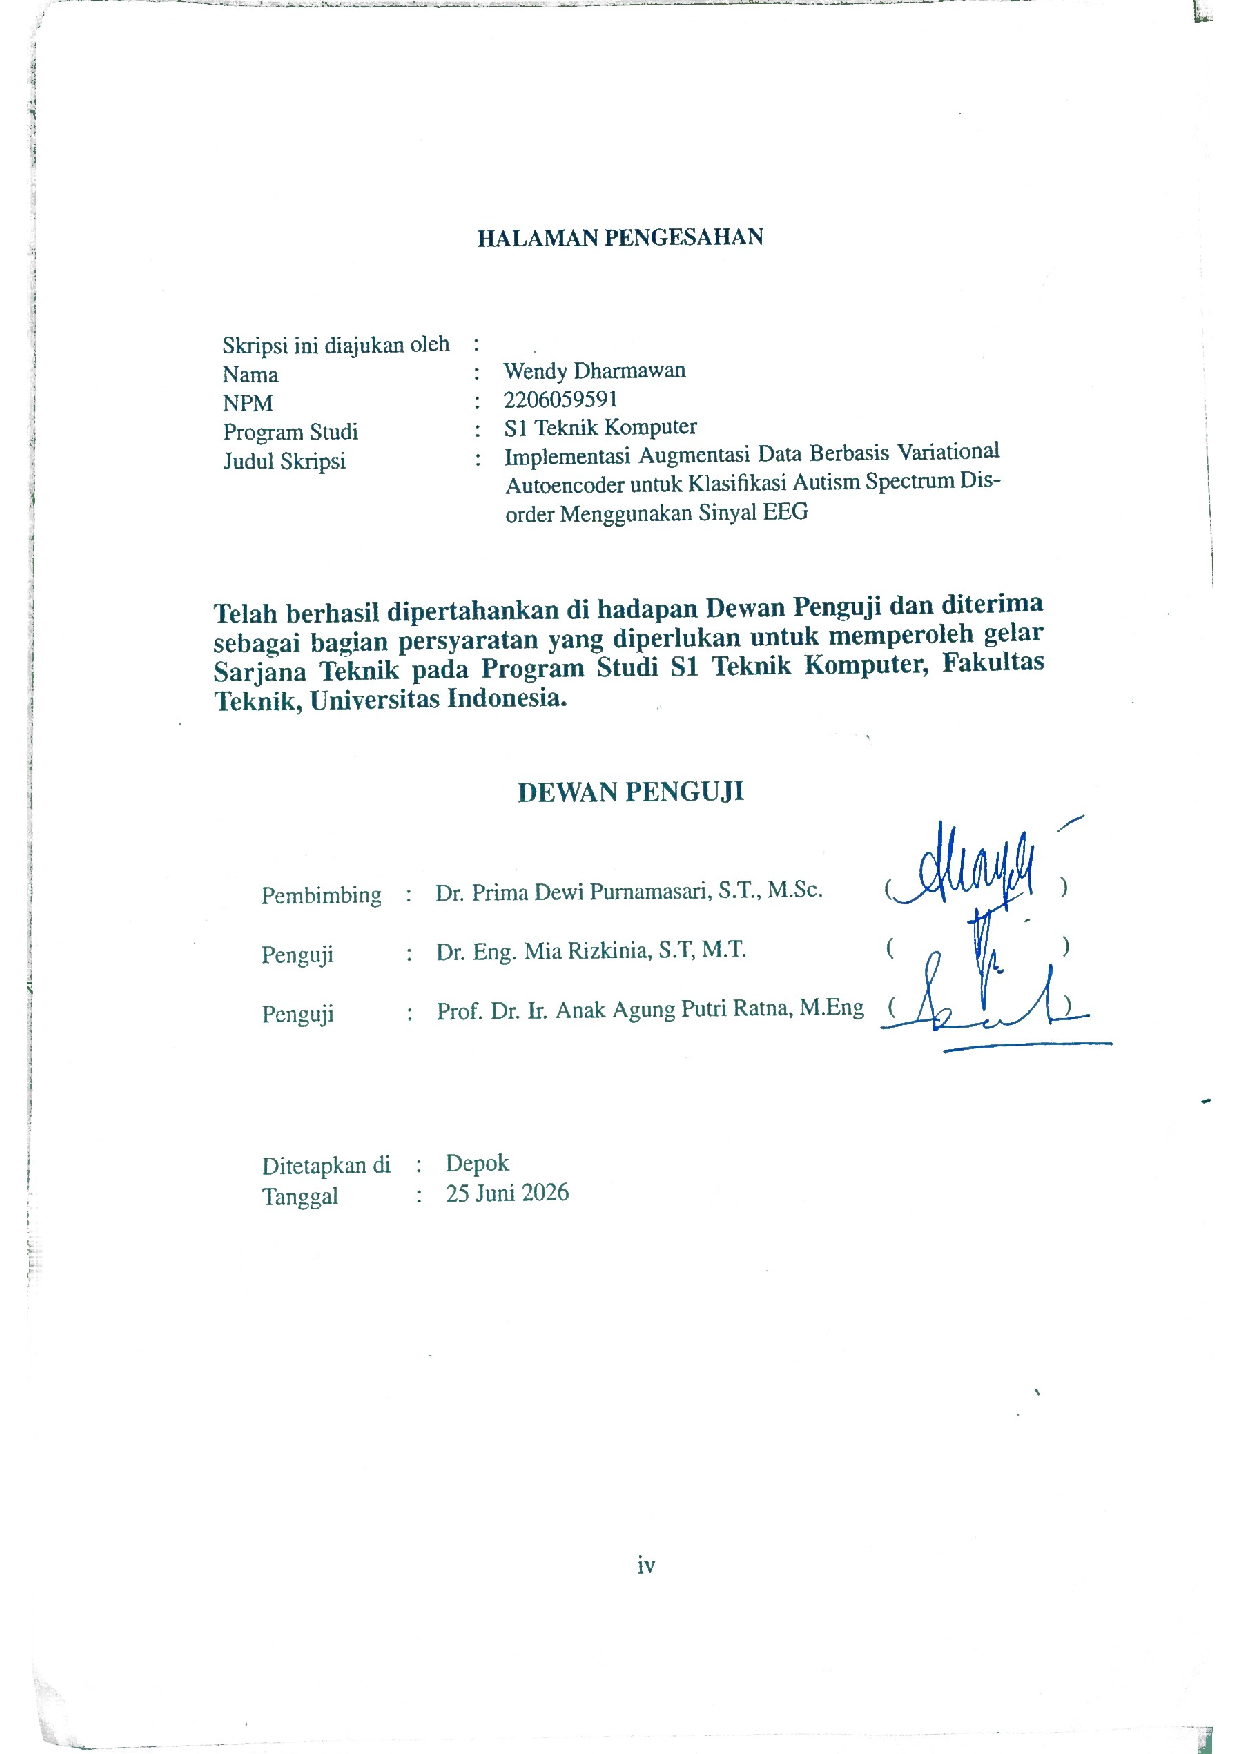
\includepdf[pages=1]{assets/pdfs/pengesahan.pdf}
%
%
\chapter*{\kataPengantar}
\thispagestyle{frontmatterNoFooter}
\addcontentsline{toc}{chapter}{\kataPengantar} % masuk daftar isi
%-----------------------------------------------------------------------------%
%\chapter*{Kata Pengantar}
\setstretch{1}
\vspace*{4\baselineskip}
\setstretch{1.5}
Puji dan syukur~\saya~panjatkan kepada Tuhan Yang Maha Esa atas berkat dan rahmat-Nya lah~\saya~dapat menyelesaikan~\type~dengan judul ``\judul''. \type~ini~\saya~laksanakan sebagai salah satu syarat dalam memperoleh gelar~\gelar~pada program studi~\program, Fakultas~\fakultas, Universitas Indonesia.

\saya\ juga ingin menyampaikan rasa terima kasihnya kepada:
\begin{enumerate}
    \item \pembimbing, selaku Dosen Pembimbing \type Penulis.
    \item \kadept, selaku Ketua Departemen Teknik Elektro, Fakultas~\fakultas, Universitas Indonesia.
    \item \kaprodi, selaku Kepala Program Studi \program, Fakultas~\fakultas, Universitas Indonesia.
    \item \pa, selaku Pembimbing Akademis Penulis.
    \item \pengujisatu,~\pengujidua~dan~\pengujitiga~selaku Dosen Penguji~\type\~Penulis.
    \item Segenap dosen Departemen Teknik Elektro atas semua ilmu yang diberikan kepada~\saya.
    \item Orang tua yang selalu memberikan dukungan serta doa, sehingga penulisan~\type~dapat diselesaikan secara baik. 
    \item Teman-teman Teknik Komputer, selaku rekan penulis yang selalu membantu serta memberikan dukungan moril sepanjang proses kuliah serta penulisan proposal skripsi.
\end{enumerate}
\saya\ menyadari dan menerima bahwa \type\ yang dibentuk ini masih jauh dari sempurna dan masih memiliki berbagai kekurangan serta kesalahan baik dari segi ilmu maupun pemahaman. Oleh karena itu, \saya\ mengharapkan segala kritik dan saran yang diberikan agar ke depannya \saya\ dapat menjadi lebih baik.

\vspace*{0.1cm}
\begin{flushright}
\tanggalPengesahan\\[0.1cm]
\vspace*{2cm}
\penulis

\end{flushright}
%
%
\setstretch{1}
\chapter*{Halaman Pernyataan Persetujuan Publikasi Tugas Akhir untuk Kepentingan Akademis}
\thispagestyle{frontmatterNoFooter}
\addcontentsline{toc}{chapter}{HALAMAN PERNYATAAN  PERSETUJUAN PUBLIKASI} % masuk daftar isi
\input{src/00-front_matter/05-persetujuan_publikasi}
%
% 
\fancypagestyle{abstrakstyle}{
    \fancyhf{} % bersihkan header/footer default
    \fancyfoot[R]{\fontsize{10}{12}\selectfont \sffamily \textbf{Universitas Indonesia}}
    \renewcommand{\headrulewidth}{0pt}
    \renewcommand{\footrulewidth}{0pt}
}

\chapter*{ABSTRAK} % judul halaman
\addcontentsline{toc}{chapter}{ABSTRAK} % masuk daftar isi
\thispagestyle{abstrakstyle} % pastikan footer diterapkan
%
% Halaman Abstrak
%
% @author  Andreas Febrian
% @version 1.00
%
%\chapter*{Abstrak}
\setstretch{1}
\vspace*{0.2cm}
%    \begingroup
    \singlespacing
	\setlength{\parindent}{0pt}
	
	\begin{tabular}{@{}l l p{10cm}}
		Nama&: & \penulis \\
		Program Studi&: & \program \\
		Judul&: & \judul \\
		Pembimbing&: & \pembimbing \\
	\end{tabular}


\bigskip
\bigskip
Autism Spectrum Disorder (ASD) merupakan gangguan perkembangan saraf yang ditandai oleh hambatan dalam komunikasi sosial dan perilaku repetitif. Berbagai penelitian telah memanfaatkan sinyal electroencephalography (EEG) untuk membantu proses klasifikasi ASD, namun keterbatasan jumlah data sering menjadi kendala dalam pengembangan model pembelajaran mesin yang andal. Penelitian ini bertujuan untuk menganalisis efektivitas augmentasi data berbasis Variational Autoencoder (VAE) dalam meningkatkan performa klasifikasi ASD menggunakan sinyal EEG. Penelitian dilakukan dengan membangun model VAE untuk menghasilkan data EEG sintetis yang kemudian digunakan sebagai data augmentasi pada proses klasifikasi. Kualitas data sintetis dievaluasi menggunakan metrik Fréchet Inception Distance (FID), Sliced Wasserstein Distance (SWD), dan normalisasi Euclidean Distance (ED), sedangkan evaluasi klasifikasi dilakukan menggunakan model Deep Neural Network (DNN) dan Extreme Gradient Boosting (XGBoost). Hasil eksperimen menunjukkan bahwa data sintetis yang dihasilkan mampu mempertahankan karakteristik utama sinyal EEG serta memberikan peningkatan performa klasifikasi. Secara signifikan, penggunaan data sintetis pada model XGBoost meningkatkan akurasi dari 97,44\% menjadi 99,54\% sensitivitas dari 97,10\% menjadi 98,67\% spesifisitas dari 97,78\% menjadi 99,96\% dan presisi dari 97,78\% menjadi 99,91\%. Temuan ini menunjukkan bahwa augmentasi berbasis VAE mampu memperkaya variasi data pelatihan dan meningkatkan kemampuan model dalam membedakan kelas ASD dan non-ASD. Penelitian ini menyimpulkan bahwa VAE merupakan pendekatan yang menjanjikan untuk mengatasi keterbatasan data EEG dan meningkatkan performa sistem klasifikasi ASD berbasis EEG.
\newline
\newline
Kata kunci: Autism Spectrum Disorder, Electroencephalography, Augmentasi Data, Variational Autoencoder, Deep Neural Network, XGBoost.

\newpage
%
%
\chapter*{ABSTRACT} % judul halaman
\addcontentsline{toc}{chapter}{ABSTRACT} % masuk daftar isi
\thispagestyle{abstrakstyle} % pastikan footer diterapkan
%
% Halaman Abstract
%
% @author  Andreas Febrian
% @version 1.00
%

%\chapter*{Abstract}
\setstretch{1}
\vspace*{0.2cm}
{
%    \begingroup
    \singlespacing
	\setlength{\parindent}{0pt}
	
	\begin{tabular}{@{}l l p{10cm}}
		Name&: & \penulis \\
		Study Program&: & \program \\
		Title&: & \judulInggris \\
		Supervisor&: & \pembimbing \\
	\end{tabular}

	\bigskip
	\bigskip

Autism Spectrum Disorder (ASD) is a neurodevelopmental disorder characterized by impairments in social communication and repetitive behavioral patterns. Numerous studies have utilized electroencephalography (EEG) signals to support ASD classification; however, the limited availability of EEG data remains a major challenge in developing reliable machine learning models. This study aims to investigate the effectiveness of Variational Autoencoder (VAE)-based data augmentation in improving ASD classification performance using EEG signals. A VAE model was developed to generate synthetic EEG data, which were subsequently used as augmented samples during the classification process. The quality of the generated synthetic data was evaluated using Fréchet Inception Distance (FID), Sliced Wasserstein Distance (SWD), and normalized Euclidean Distance (ED), while classification performance was assessed using Deep Neural Network (DNN) and Extreme Gradient Boosting (XGBoost) models. Experimental results demonstrate that the synthetic data generated by the VAE preserve the main characteristics of the original EEG signals while improving classification performance. In particular, the use of synthetic data in the XGBoost model increased accuracy from 97.44\% to 99.51\%, sensitivity from 97.24\% to 98.79\%, specificity from 97.86\% to 99.86\%, and precision from 97.51\% to 99.70\%. These findings indicate that VAE-based augmentation can enrich training data diversity and enhance the model's ability to distinguish between ASD and non-ASD classes. This study concludes that VAE is a promising approach for addressing EEG data limitations and improving the performance of EEG-based ASD classification systems.

	\bigskip

	Keywords:
	Autism Spectrum Disorder, Electroencephalography, Data Augmentation, Variational Autoencoder, Deep Neural Network, XGBoost.
%    \endgroup
}

\newpage

%
% Daftar isi, gambar, dan tabel
%
\phantomsection
\begingroup
\singlespacing
% --- Aktifkan footer mulai dari sini ---
% Frontmatter style (plain)
\pagestyle{plain}  % Untuk seluruh frontmatter
\tableofcontents
\clearpage
\phantomsection
\listoftables
\clearpage
\phantomsection
\listoffigures
\clearpage
\phantomsection
\addcontentsline{toc}{chapter}{DAFTAR PERSAMAAN}
\listofequs
\clearpage
\phantomsection
\input{src/00-front_matter/daftar-notasi}%Jika diperlukan
\clearpage
%\phantomsection
%\addcontentsline{toc}{chapter}{DAFTAR ISTILAH}
%\printnomenclature%Jika diperlukan
%\clearpage
\phantomsection
\addcontentsline{toc}{chapter}{\listlistingname}
\listoflistings%Jika diperlukan
\clearpage
\phantomsection
\addcontentsline{toc}{chapter}{\listabbreviationname}
%\listofabbreviation%Jika diperlukan
%\printacronyms
\chapter*{DAFTAR SINGKATAN}
\begin{acronym}[minimum Redundancy Maximum Relevance]
    \acro{ASD}{\textit{Autism Spectrum Disorder}}
    \acro{BCI}{\textit{Brain--Computer Interface}}
    \acro{CNN}{\textit{Convolutional Neural Network}}
    \acro{DWT}{\textit{Discrete Wavelet Transform}}
    \acro{EEG}{\textit{Electroencephalography}}
    \acro{ELBO}{\textit{Evidence Lower Bound}}
    \acro{EMG}{\textit{Electromyogram}}
    \acro{EOG}{\textit{Electrooculogram}}
    \acro{FFT}{\textit{Fast Fourier Transform}}
    \acro{GAN}{\textit{Generative Adversarial Network}}
    \acro{ICA}{\textit{Independent Component Analysis}}
    \acro{kNN}{\textit{k-Nearest Neighbor}}
    \acro{KL}{\textit{Kullback--Leibler}}
    \acro{mRMR}{\textit{Minimum Redundancy Maximum Relevance}}
    \acro{PSD}{\textit{Power Spectral Density}}
    \acro{SNR}{\textit{Signal-to-Noise Ratio}}
    \acro{SVM}{\textit{Support Vector Machine}}
    \acro{VAE}{\textit{Variational Autoencoder}}
\end{acronym}


\clearpage
\endgroup

%
% Gunakan penomeran Arab (1, 2, 3, ...) setelah bagian ini.
%
\pagenumbering{arabic}

%
%
%
% Setelah cover, kata pengantar, abstrak, Daftar Isi
\pagestyle{fancy}
\fancyhf{}
\fancyhead[R]{\thepage} % nomor halaman kanan atas
\fancyfoot[R]{\fontsize{10}{12}\selectfont \sffamily \textbf{Universitas Indonesia}}
\renewcommand{\headrulewidth}{0pt}
\renewcommand{\footrulewidth}{0pt}

\setstretch{1.5} % <-- double spacing
\setlength{\parindent}{1.5em}

%-----------------------------------------------------------------------------%
\chapter{\babSatu}
\label{Pendahuluan}
%-----------------------------------------------------------------------------%
Autism Spectrum Disorder (ASD) merupakan gangguan neurologis yang memengaruhi komunikasi, interaksi sosial, dan perilaku individu, sehingga proses identifikasi dini memiliki peranan penting dalam penanganannya. Analisis sinyal electroencephalography (EEG) menggunakan metode machine learning mulai banyak diteliti sebagai pendekatan dalam proses klasifikasi ASD secara lebih objektif. Meskipun demikian, pengembangan model klasifikasi berbasis EEG masih menghadapi tantangan berupa keterbatasan dataset EEG yang tersedia dan tingginya variabilitas sinyal antar individu maupun antar sesi perekaman. Karakteristik tersebut menyebabkan terhambatnya proses pengembangan model klasifikasi EEG yang mampu memberikan performa secara konsisten pada data dengan karakteristik yang berbeda. Salah satu pendekatan yang mulai banyak digunakan untuk mengatasi permasalahan tersebut adalah teknik \textit{data augmentation}, yaitu proses penambahan variasi data \textit{training} secara artifisial, sehingga diharapkan dapat meningkatkan performa dan kemampuan generalisasi model.

Bab ini akan dimulai dengan penjelasan Latar Belakang yang memberikan konteks penting terkait penelitian ini, diikuti oleh Rumusan Masalah dan Tujuan Penelitian yang merinci fokus utama studi. Selanjutnya, akan dibahas Manfaat Penelitian dan Ruang Lingkup Penelitian untuk menjelaskan kontribusi serta batasan penelitian ini. Terakhir, Sistematika Penulisan akan menguraikan struktur keseluruhan laporan penelitian.

%-----------------------------------------------------------------------------%
\section{Latar Belakang}
\label{sec:latar_belakang}
%-----------------------------------------------------------------------------%

Autism Spectrum Disorder (ASD) merupakan gangguan neurologis yang ditandai oleh hambatan dalam komunikasi dan interaksi sosial, serta pola perilaku yang terbatas dan berulang \cite{nih_autism}, \cite{dsm5}. Identifikasi dan intervensi dini menjadi faktor penting dalam membantu perkembangan individu dengan ASD, namun proses diagnosis masih menghadapi berbagai tantangan karena karakteristik gejala yang heterogen dan sering kali menyerupai gangguan perkembangan lainnya \cite{autism_diagnosis_challenges} \cite{10423494}. Kondisi tersebut mendorong berkembangnya pendekatan diagnosis berbasis biomarker yang lebih objektif dan konsisten.

Salah satu pendekatan yang banyak diteliti adalah analisis electroencephalography (EEG) menggunakan metode machine learning. Dibandingkan dengan metode lainnya, EEG memiliki keunggulan karena bersifat non-invasif, relatif lebih murah, dan memiliki resolusi temporal yang tinggi \cite{brain_imaging_asd_review} \cite{eeg_dataset_asd}. Berbagai penelitian menunjukkan bahwa model machine learning mampu mengidentifikasi pola aktivitas otak yang berkaitan dengan ASD melalui sinyal EEG dengan performa klasifikasi yang cukup baik \cite{eeg_autism_review}. Penelitian rujukan \cite{paper_ref} mengusulkan pendekatan klasifikasi ASD berbasis EEG menggunakan kombinasi seleksi fitur minimum Redundancy Maximum Relevance (mRMR) dan algoritma XGBoost yang menunjukkan performa klasifikasi yang baik dan konsisten.

Meskipun demikian, pengembangan model klasifikasi EEG masih menghadapi berbagai tantangan, terutama terkait keterbatasan dataset EEG yang tersedia secara publik dan telah memiliki label klinis \cite{dl_eeg_review}. Proses akuisisi dan pelabelan data EEG umumnya membutuhkan biaya, waktu, serta keterlibatan tenaga ahli, sehingga jumlah data yang tersedia sering kali terbatas. Keterbatasan dataset ini dapat meningkatkan risiko overfitting pada proses training model machine learning dan membatasi kemampuan model dalam melakukan generalisasi terhadap data baru \cite{eeg_limited_data}. Selain itu, sinyal EEG juga rentan terhadap berbagai artefak, seperti gerakan otot, kedipan mata, maupun gangguan pada perangkat perekaman yang dapat memengaruhi kualitas sinyal \cite{artifact_removal_eeg}. Keberadaan artefak tersebut menyebabkan proses analisis EEG menjadi lebih sulit karena sinyal yang diperoleh tidak selalu merepresentasikan aktivitas otak yang sebenarnya.

Salah satu pendekatan yang mulai banyak diteliti untuk mengatasi keterbatasan dataset EEG adalah penggunaan teknik data augmentation. Teknik ini bertujuan untuk meningkatkan jumlah dan variasi data training secara artifisial sehingga model dapat mempelajari representasi fitur yang lebih beragam. Beberapa penelitian menunjukkan bahwa penerapan data augmentation pada data EEG dapat membantu meningkatkan performa model klasifikasi dan mengurangi risiko overfitting pada kondisi dataset yang terbatas \cite{eeg_augmentation_review}.

Penerapan augmentasi pada data EEG memiliki tantangan tersendiri karena sinyal EEG merupakan data \textit{time series} multikanal yang bersifat non-stasioner dan memiliki rasio \textit{signal-to-noise} yang rendah \cite{eeg_feature_review}. Berbeda dengan berbagai jenis data multimedia lain seperti citra, audio, atau video yang umumnya memiliki pola representasi yang lebih stabil, manipulasi pada data EEG perlu dilakukan secara hati-hati karena perubahan pada sinyal dapat memengaruhi representasi aktivitas otak yang dianalisis. Pendekatan augmentasi data konvensional pada data \textit{time series} umumnya dilakukan melalui transformasi sederhana seperti penambahan \textit{noise}, pergeseran waktu, atau manipulasi amplitudo. Namun, pada data EEG, transformasi tersebut berpotensi mengubah karakteristik temporal dan spasial yang digunakan dalam proses analisis maupun klasifikasi sinyal \cite{gan_eeg_emotion}.

Seiring dengan perkembangan deep learning, pendekatan berbasis model generatif seperti Variational Autoencoder (VAE) mulai digunakan untuk menghasilkan data EEG sintetis yang lebih representatif. Model VAE mempelajari distribusi laten dari data EEG sehingga mampu menghasilkan sampel baru yang berbeda namun tetap mempertahankan karakteristik statistik dari data asli. Pendekatan generatif memiliki potensi untuk menghasilkan variasi data yang lebih realistis dibandingkan metode augmentasi konvensional \cite{gan_eeg_emotion}. Meskipun demikian, pemanfaatan data sintetis berbasis model generatif pada klasifikasi EEG, khususnya dalam konteks Autism Spectrum Disorder (ASD), masih memerlukan kajian lebih lanjut untuk memahami pengaruhnya terhadap performa dan kemampuan generalisasi model klasifikasi.

Berdasarkan permasalahan tersebut, penelitian ini bertujuan untuk mengeksplorasi penggunaan teknik data augmentation berbasis Variational Autoencoder (VAE) untuk menghasilkan data EEG sintetis dan menganalisis pengaruhnya terhadap performa model klasifikasi ASD berbasis EEG. 
\section{Rumusan Masalah}
\label{sec:rumusan_masalah}
%-----------------------------------------------------------------------------%
Berdasarkan latar belakang yang telah dijelaskan, permasalahan utama dalam penelitian
ini dirumuskan sebagai berikut:
\begin{enumerate}
    \item Bagaimana pendekatan yang dapat digunakan untuk mengatasi keterbatasan jumlah dan variasi data pada sinyal EEG dalam konteks klasifikasi Autism Spectrum Disorder (ASD)?
    
    \item Sejauh mana data sintetis yang dihasilkan melalui proses augmentasi mampu mempertahankan karakteristik dan distribusi sinyal EEG asli?
    
    \item Bagaimana pengaruh penggunaan data hasil augmentasi terhadap performa dan kemampuan generalisasi model klasifikasi EEG dalam mendeteksi pola yang berkaitan dengan Autism Spectrum Disorder (ASD)?
\end{enumerate}

%-----------------------------------------------------------------------------%
\section{Tujuan Penelitian}
\label{sec:tujuan_penelitian}
%-----------------------------------------------------------------------------%

Selaras dengan rumusan masalah yang telah diuraikan, tujuan dari penelitian ini mencakup sebagai berikut:

\begin{enumerate}
    \item Mengkaji dan mengidentifikasi pendekatan yang dapat digunakan untuk mengatasi keterbatasan jumlah dan variasi data pada sinyal EEG dalam konteks klasifikasi Autism Spectrum Disorder (ASD).

    \item Mengevaluasi sejauh mana data sintetis yang dihasilkan melalui proses augmentasi mampu mempertahankan karakteristik dan distribusi sinyal EEG asli.

    \item Menganalisis pengaruh penggunaan data hasil augmentasi terhadap performa serta kemampuan generalisasi model klasifikasi EEG dalam mendeteksi pola yang berkaitan dengan Autism Spectrum Disorder (ASD).
\end{enumerate}

%-----------------------------------------------------------------------------%
\section{Manfaat Penelitian}
\label{sec:manfaat_penelitian}
%-----------------------------------------------------------------------------%
Berdasarkan latar belakang, rumusan masalah, dan tujuan penelitian yang telah diuraikan, penelitian ini diharapkan memberikan manfaat sebagai berikut:

\begin{enumerate}
    \item \textbf{Bagi Peneliti dan Pengembangan Metode:} \\
    Penelitian ini diharapkan dapat menjadi referensi dalam pengembangan dan pemanfaatan teknik \textit{data augmentation} pada sinyal EEG, serta membuka peluang bagi pengembangan metode klasifikasi dan diagnosis di masa depan yang mampu memanfaatkan data dalam jumlah yang lebih besar dan beragam, sehingga meningkatkan robustness dan kemampuan generalisasi model.

    \item \textbf{Bagi Tenaga Medis dan Profesional Kesehatan:} \\
    Penelitian ini diharapkan dapat memberikan gambaran mengenai potensi pemanfaatan \textit{machine learning} dalam analisis data EEG pada studi Autism Spectrum Disorder (ASD), maupun untuk  sehingga dapat mendukung pemahaman dan penelitian lanjutan terkait pendekatan berbasis data dalam konteks klinis.
\end{enumerate}

%-----------------------------------------------------------------------------%
\section{Ruang Lingkup Penelitian}
\label{sec:ruang_lingkup}
%-----------------------------------------------------------------------------%
Agar penelitian ini tetap terfokus, maka ruang lingkup penelitian ditetapkan sebagai berikut:
\begin{enumerate}

\item \textbf{Dataset Penelitian:} Penelitian ini menggunakan dataset EEG yang sama dengan dataset pada penelitian rujukan \cite{paper_ref}\cite{eeg_dataset_asd}. Dataset tersebut digunakan sebagai dasar dalam proses pelatihan model augmentasi maupun model klasifikasi sehingga hasil penelitian dapat dibandingkan secara relevan dengan penelitian sebelumnya.

\item \textbf{Metode Preprocessing Data:} Tahapan \textit{preprocessing} data EEG mengikuti prosedur yang digunakan pada penelitian rujukan \cite{paper_ref}. Proses ini mencakup tahapan pengolahan data yang diperlukan sebelum proses seleksi fitur, augmentasi data, dan klasifikasi dilakukan.

\item \textbf{Metode Augmentasi dan Klasifikasi:} Penelitian ini menerapkan metode \textit{data augmentation} berbasis \textit{Variational Autoencoder} (VAE) untuk menghasilkan data EEG sintetis. Selanjutnya, proses klasifikasi dilakukan menggunakan pendekatan yang mengacu pada penelitian rujukan \cite{paper_ref}, yaitu kombinasi seleksi fitur \textit{mRMR} dan model klasifikasi \textit{XGBoost}.

\item \textbf{Metode Evaluasi:} Evaluasi penelitian dilakukan dengan membandingkan performa model klasifikasi pada data tanpa augmentasi dan dengan augmentasi. Penilaian kualitas data sintetis serta performa klasifikasi mengacu pada metode evaluasi yang digunakan dalam penelitian rujukan \cite{eeg_gan}.

\item \textbf{Hasil Akhir Penelitian:} Penelitian ini menghasilkan model \textit{data augmentation} EEG berbasis \textit{Variational Autoencoder} (VAE) yang dapat digunakan untuk menghasilkan data EEG sintetis guna mendukung peningkatan performa model klasifikasi.


\item \textbf{Batasan Penelitian:} Penelitian difokuskan pada analisis pengaruh penerapan \textit{data augmentation} EEG terhadap kualitas performa model klasifikasi. Penelitian ini tidak membahas aspek perangkat keras EEG, proses akuisisi data asli, maupun tahapan penghilangan \textit{noise} dan \textit{artifact removal} di luar prosedur \textit{preprocessing} yang telah ditetapkan pada penelitian rujukan.
\end{enumerate}
%-----------------------------------------------------------------------------%
\section{Sistematika Penulisan}
\label{sec:sistematika}
%-----------------------------------------------------------------------------%
Laporan tesis ini disusun secara sistematis ke dalam lima bab utama, dengan rincian se-
bagai berikut:

\begin{enumerate}
    \item \textbf{Bab 1: Pendahuluan.} 
    Bab ini menyajikan gambaran umum penelitian, meliputi latar belakang yang menjelaskan pentingnya analisis sinyal EEG dalam mendukung identifikasi Autism Spectrum Disorder (ASD), rumusan masalah yang menjadi dasar penelitian, tujuan yang ingin dicapai, manfaat penelitian, ruang lingkup penelitian, serta sistematika penulisan laporan ini.
    
    \item \textbf{Bab 2: Tinjauan Pustaka.} 
    Bab ini menguraikan landasan teoretis yang mendukung penelitian, meliputi konsep dasar sinyal EEG, metode ekstraksi dan seleksi fitur pada data EEG, metode \textit{Minimum Redundancy Maximum Relevance} (mRMR), implementasi \textit{machine learning}  dalam klasifikasi berdasarkan EEG, metode augmentasi data EEG, model \textit{Variational AutoEncoder}, serta kajian terhadap penelitian-penelitian sebelumnya yang bersifat relevan.
    
    \item \textbf{Bab 3: Metodologi Penelitian.} 
    Bab ini menjelaskan metode yang digunakan dalam penelitian, mencakup deskripsi dataset EEG yang digunakan, tahapan pra-pemrosesan data, penerapan teknik \textit{data augmentation}, proses seleksi fitur menggunakan metode \textit{mRMR}, arsitektur model augmentasi berbasis \textit{VAE}, serta konfigurasi \textit{training} model klasifikasi menggunakan \textit{XGBoost}.
    
    \item \textbf{Bab 4: Hasil dan Analisis.} 
    Bab ini memaparkan hasil eksperimen yang diperoleh dari proses \textit{training} dan pengujian model. Analisis dilakukan untuk membandingkan performa model pada skenario dengan dan tanpa penerapan \textit{data augmentasi}, serta mengevaluasi pengaruhnya terhadap kemampuan model dalam melakukan klasifikasi data EEG.
    
    \item \textbf{Bab 5: Penutup.} 
    Bab terakhir ini berisi kesimpulan dari hasil penelitian yang telah dilakukan serta saran untuk pengembangan penelitian selanjutnya terkait analisis dan klasifikasi data EEG menggunakan metode \textit{machine learning} .
\end{enumerate}
%-----------------------------------------------------------------------------%
\chapter{\babDua}
\label{cha:Tinjauan Pustaka}
%-----------------------------------------------------------------------------%
Bab ini menjelaskan konteks dan landasan teoretis yang mendasari penelitian mengenai analisis sinyal EEG untuk klasifikasi \textit{Autism Spectrum Disorder} (ASD) menggunakan metode \textit{machine learning}. Penjelasan diawali dengan pemaparan landasan teori, dilanjutkan dengan pembahasan penelitian terdahulu yang relevan, dan diakhiri dengan pembahasan mengenai celah penelitian yang menjadi dasar penelitian ini.
\section{Landasan Teori}
\label{sec:landasan_teori}
Bagian ini menguraikan konsep-konsep teoretis yang menjadi dasar dalam penelitian analisis sinyal EEG untuk klasifikasi Autism Spectrum Disorder (ASD). Landasan teori ini mencakup konsep dasar EEG, tahapan pemrosesan sinyal EEG, teknik seleksi fitur dalam pemrosesan, metode \textit{machine learning} untuk klasifikasi, serta metode \textit{data augmentation} yang digunakan dalam penelitian ini.

\subsection{Sinyal EEG}
\label{Konsep Dasar Sinyal EEG}

Sinyal \textit{electroencephalogram} (EEG) dihasilkan oleh aktivitas listrik neuron di otak yang muncul akibat aktivitas sinaptik antar neuron, sehingga potensial listrik yang dihasilkan dapat dideteksi pada permukaan kepala menggunakan elektroda. Sinyal EEG direkam sebagai perubahan tegangan terhadap waktu dengan rentang frekuensi sekitar 0,5 hingga 100 Hz dan amplitudo yang relatif rendah, umumnya berada pada kisaran 10 hingga 100 mikrovolt. Selain memiliki resolusi temporal yang tinggi, sinyal EEG juga bersifat \textit{non-stationary}, sehingga karakteristik amplitudo dan distribusi frekuensinya dapat berubah secara dinamis seiring waktu akibat pengaruh kondisi fisiologis, tingkat kesadaran, maupun aktivitas kognitif. Aktivitas yang terekam mencerminkan berbagai proses otak, seperti fungsi kognitif, motorik, dan emosional, sehingga EEG banyak digunakan untuk mempelajari fungsi otak dan gangguan neurologis \cite{eeg_basics}.

EEG biasanya direkam dalam bentuk sinyal multikanal yang diperoleh dari sejumlah elektroda yang ditempatkan pada berbagai lokasi di permukaan kulit kepala. Setiap kanal merepresentasikan satu jalur perekaman sinyal yang berasal dari pasangan elektroda atau dari elektroda terhadap referensi tertentu. Setiap elektroda menangkap aktivitas listrik dari wilayah otak yang berbeda, sehingga setiap kanal mengandung informasi yang merepresentasikan aktivitas saraf pada lokasi tertentu.\cite{eeg_feature_review}.


Penempatan elektroda EEG umumnya mengikuti standar International \textit{10–20 System}, yaitu protokol yang distandarisasi oleh \textit{International Federation of Clinical Neurophysiology} (IFCN) untuk menentukan posisi elektroda pada permukaan kepala berdasarkan titik anatomi seperti nasion, inion, dan titik preauricular. Dalam sistem ini, setiap elektroda diberi kode huruf dan angka yang menunjukkan wilayah otak dan hemisfer terkait, seperti frontal (F), central (C), temporal (T), parietal (P), dan occipital (O), dengan angka ganjil untuk hemisfer kiri, angka genap untuk hemisfer kanan, serta ``z'' untuk posisi garis tengah kepala. Tata letak elektroda pada sistem ini ditunjukkan pada Gambar \ref{fig:2.1}. Standarisasi ini memungkinkan perekaman EEG dilakukan secara konsisten dan dapat dibandingkan antar subjek maupun antar penelitian\cite{eeg_biophysics}.

\begin{figure}[H]
    \centering
    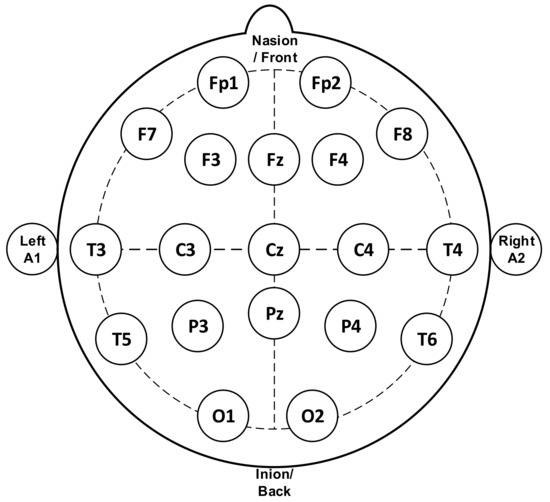
\includegraphics[width=0.6\textwidth]{assets/pics/10_20_system.jpg}
    \caption{Sistem Internasional 10--20 untuk penempatan elektroda EEG}
    \label{fig:2.1}
\end{figure}

Dalam analisis sinyal EEG, aktivitas listrik otak yang terekam dapat dianalisis melalui dua domain utama, yaitu domain waktu dan domain frekuensi. Analisis dalam domain waktu dilakukan dengan mengamati karakteristik sinyal terhadap waktu, seperti amplitudo puncak, dan latensi. Sedangkan analisis dalam domain frekuensi bertujuan untuk mengidentifikasi kandungan spektral sinyal dengan memeriksa distribusi energi atau daya pada berbagai rentang frekuensi menggunakan metode transformasi spektral, seperti \textit{Fast Fourier Transform} (FFT) maupun teknik estimasi \textit{Power Spectral Density} (PSD) untuk mengidentifikasi aktivitas otak pada rentang frekuensi tertentu \cite{auditory_eeg}.

Dalam analisis spektral EEG, sinyal umumnya dibagi ke dalam beberapa segmen waktu (\textit{epoch}) sebelum dihitung nilai \textit{Power Spectral Density} (PSD) untuk menggambarkan distribusi daya pada setiap frekuensi. Berdasarkan karakteristik fisiologis dan kognitifnya, sinyal EEG kemudian diklasifikasikan ke dalam beberapa pita frekuensi utama seperti pada tabel \ref{tab:eeg_bands}.

\begin{table}[H]
\centering
\footnotesize
\caption{Pita frekuensi EEG dan karakteristiknya}
\label{tab:eeg_bands}
\begin{tabular}{|c|c|p{8cm}|}
\hline
\textbf{Pita} & \textbf{Frekuensi (Hz)} & \textbf{Karakteristik} \\ \hline
Delta & 0,5--4 & Dominan pada kondisi \textit{deep sleep} dan berperan dalam proses pemulihan fisiologis serta regulasi fungsi tubuh selama tidur. \\ \hline
Theta & 4--8 & Berkaitan dengan proses pembentukan memori dan aktivitas pada sistem limbik serta hipokampus, serta muncul pada kondisi mengantuk atau relaksasi mendalam. \\ \hline
Alpha & 8--13 & Muncul pada kondisi rileks saat mata tertutup, dengan dominasi pada wilayah oksipital dan berhubungan dengan penurunan aktivitas pemrosesan sensorik. \\ \hline
Beta & 13--30 & Berkaitan dengan aktivitas kognitif aktif seperti konsentrasi, pemecahan masalah, serta aktivitas motorik. \\ \hline
Gamma & >30 & Berhubungan dengan proses kognitif tingkat tinggi, termasuk perhatian, integrasi informasi sensorik, dan persepsi. \\ \hline
\end{tabular}
\end{table}
Melalui analisis distribusi daya pada pita frekuensi, dapat dilakukan identifikasi pola aktivitas otak yang khas serta membandingkan karakteristik sinyal EEG pada berbagai kondisi fisiologis maupun gangguan neurologis tertentu. Representasi pita frekuensi EEG sering digunakan sebagai dasar dalam proses ekstraksi fitur pada analisis sinyal EEG, misalnya melalui perhitungan \textit{band power}, estimasi \textit{power spectral density} (PSD), maupun metode analisis spektral lainnya \cite{eeg_feature_review}. Rentang pita frekuensi EEG beserta posisinya pada spektrum frekuensi rendah hingga tinggi ditunjukkan pada ilustrasi \ref{fig:2.2}.

\begin{figure}[H]
    \centering
    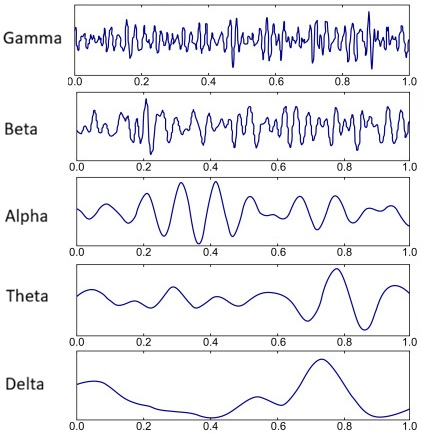
\includegraphics[width=0.6\textwidth]{assets/pics/frequency_band.png}
    \caption{Pita Frekuensi EEG pada rentang frekuensi tinggi dan rendah}
    \label{fig:2.2z}
\end{figure}
 

Sebelum dilakukan ekstraksi fitur dan klasifikasi, sinyal EEG umumnya melalui tahap \textit{preprocessing} untuk meningkatkan kualitas sinyal dan mengurangi gangguan yang tidak relevan. Tahapan ini biasanya meliputi \textit{filtering}, \textit{artifact removal}, \textit{baseline correction}, serta normalisasi atau standarisasi data \cite{eeg_feature_review}.


\textit{Filtering} adalah proses penyaringan sinyal untuk menghilangkan komponen frekuensi yang tidak berkaitan dengan aktivitas saraf serta mengurangi gangguan dari lingkungan seperti interferensi listrik serta gangguan yang muncul akibat pergerakan elektroda dan perubahan impedansi kulit. \textit{Filtering} dilakukan dengan membatasi rentang frekuensi sinyal menggunakan filter tertentu. Umumnya, \textit{band-pass filter} digunakan untuk mempertahankan frekuensi aktivitas otak, serta \textit{notch filter} untuk mereduksi interferensi jaringan listrik. Filter tambahan seperti \textit{high-pass filter} juga dapat digunakan untuk menghilangkan \textit{drift} sinyal berfrekuensi sangat rendah, sedangkan \textit{low-pass filter} digunakan untuk mereduksi komponen \textit{noise} berfrekuensi tinggi. Pemilihan filter perlu dilakukan secara hati-hati untuk menghindari distorsi sinyal atau pergeseran fase sinyal \cite{eeg_feature_review}. Pengaruh penggunaan filter terhadap sinyal EEG dapat dilihat pada ilustrasi \ref{fig:2.2}.


\begin{figure}[H]
    \centering
    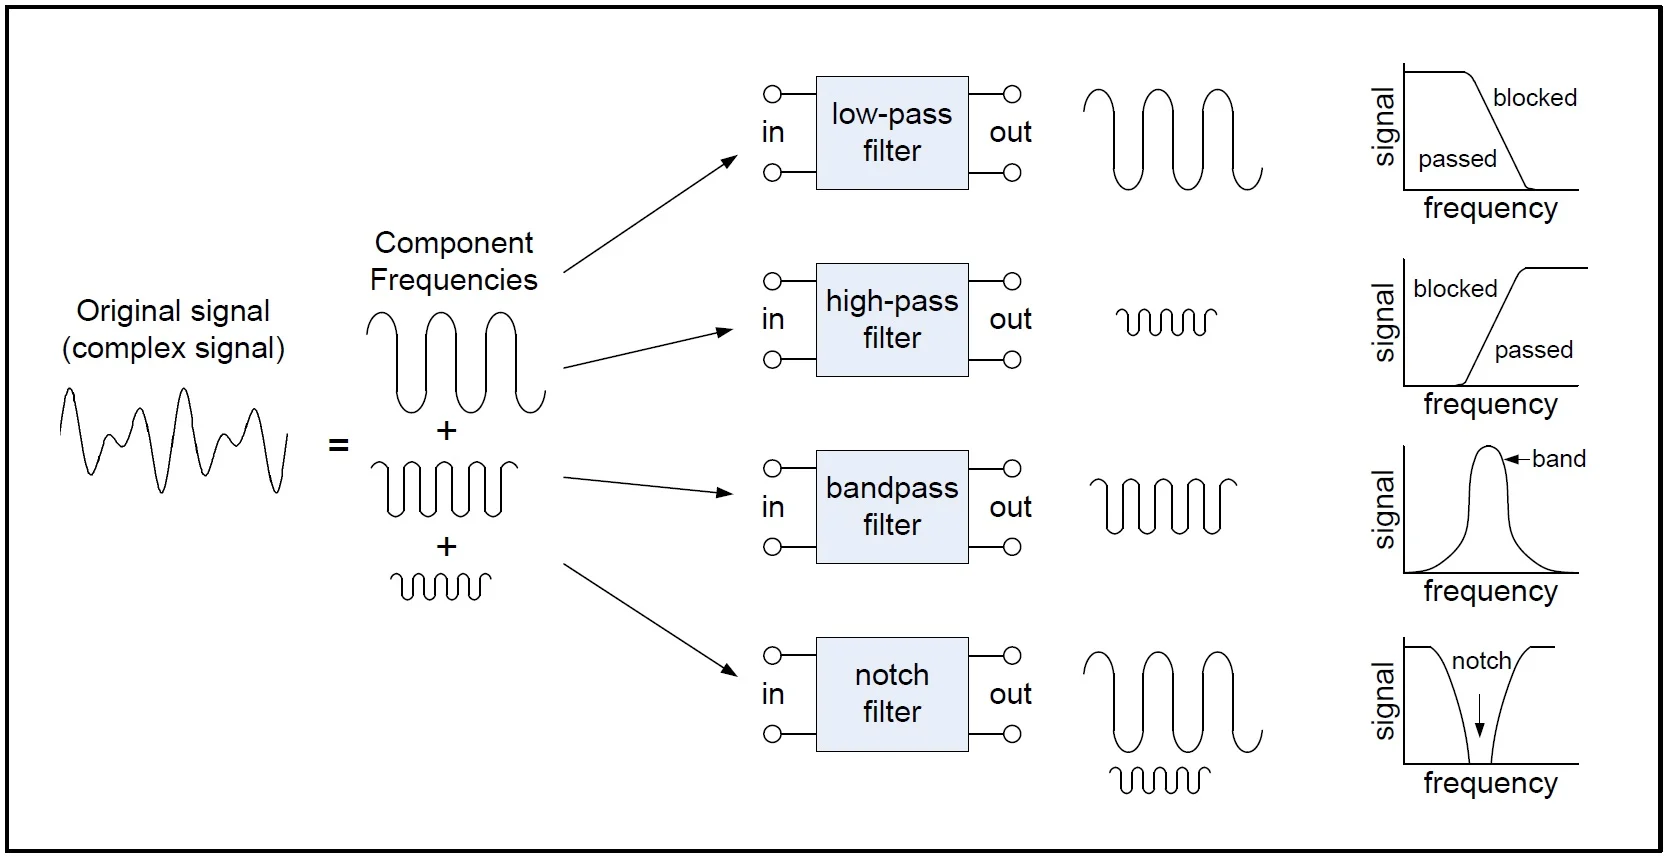
\includegraphics[width=\textwidth]{assets/pics/four_major_filters.png}
    \caption{Ilustrasi pengaruh berbagai jenis filter terhadap sinyal EEG}
    \label{fig:2.2}
\end{figure}

Sinyal EEG dapat terkontaminasi oleh artefak non-neural yang berasal dari aktivitas fisiologis maupun faktor eksternal. Artefak fisiologis umumnya disebabkan oleh kedipan mata dan pergerakan bola mata (\textit{electrooculogram}) dan aktivitas otot wajah dan kepala (\textit{electromyogram}), sedangkan artefak eksternal dapat berasal dari interferensi perangkat elektronik dan jaringan listrik. Keberadaan artefak dapat mempengaruhi kualitas sinyal, sebagaimana yang terlihat pada \ref{fig:2.3}, sehingga berpotensi menurunkan akurasi analisis maupun kinerja sistem klasifikasi. Berbagai metode digunakan untuk mengurangi artefak pada sinyal EEG, seperti \textit{Blind Source Separation} (BSS), \textit{Independent Component Analysis} (ICA), serta transformasi wavelet yang memungkinkan analisis pada domain waktu dan frekuensi untuk mendeteksi artefak \cite{eeg_feature_review}.

\begin{figure}[H]
    \centering
    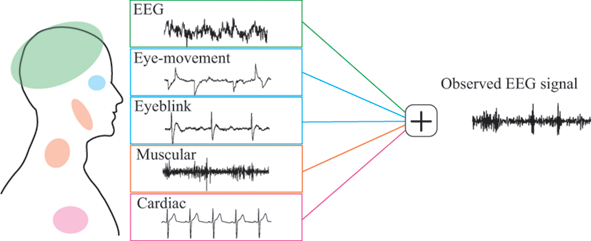
\includegraphics[width=0.6\textwidth]{assets/pics/artifact_eeg.png}
    \caption{Bentuk-Bentuk artefak pada sinyal EEG}
    \label{fig:2.3}
\end{figure}

Dalam analisis EEG berbasis \textit{machine learning}, normalisasi atau standarisasi digunakan untuk mengurangi variasi antar kanal maupun antar subjek yang menyebabkan perbedaan skala fitur dan mempengaruhi proses \textit{training}. Proses normalisasi digunakan untuk menyesuaikan skala fitur agar berada dalam rentang yang lebih seragam. Salah satu metode yang umum digunakan adalah \textit{Z-score normalization}, yaitu mengurangkan nilai rata-rata dan membaginya dengan standar deviasi sehingga data memiliki rata-rata nol dan variansi satu, sedangkan \textit{min-max normalization} juga dapat dilakukan dengan menskalakan nilai fitur ke dalam rentang tertentu, umumnya antara 0 dan 1. Proses ini memastikan kontribusi fitur lebih seimbang serta meningkatkan stabilitas dan kinerja model \cite{eeg_feature_review}.

\subsection{Feature Selection mRMR}
\label{Feature Selection mRMR}
Dalam aplikasi klasifikasi \textit{machine learning}, \textit{feature selection} merupakan langkah krusial untuk meminimalkan kesalahan klasifikasi. Secara formal, diberikan dataset $D$ yang terdiri dari $N$ sampel dan $M$ fitur $X = \{x_i \mid i = 1, 2, \dots, M\}$, serta variabel target $c$, maka seleksi fitur bertujuan menentukan subset berdimensi lebih rendah $R^m \subset R^M$ dengan $m < M$ yang mampu merepresentasikan target secara optimal\cite{mrmr_original}.

Secara umum, tujuan \textit{feature selection} dapat diformulasikan sebagai proses optimasi untuk mencari himpunan fitur $S \subseteq X$ dengan $|S| = m$ yang memaksimalkan ketergantungan terhadap kelas target. Ketergantungan ini seringkali diukur menggunakan \textit{mutual information} $I(S; c)$, sehingga permasalahan dapat dinyatakan sebagai:
\begin{equation}
\max_{S \subseteq X, |S| = m} I(S; c)
\end{equation}

Penggunaan seluruh fitur tidak selalu menghasilkan performa optimal karena adanya redundansi antar fitur. Fitur dengan korelasi tinggi cenderung memberikan informasi yang berulang, sehingga diperlukan metode \textit{feature selection} yang mempertimbangkan relevansi terhadap target sekaligus meminimalkan redundansi.

\textit{Minimum Redundancy Maximum Relevance} (mRMR) merupakan teknik seleksi fitur berbasis teori informasi yang memilih subset fitur dengan relevansi tinggi terhadap target dan redundansi rendah antar fitur.  Pendekatan ini efektif dalam mengurangi dimensi data tanpa mengorbankan informasi penting, sehingga meningkatkan efisiensi komputasi dan kemampuan generalisasi model \cite{sleep_apnea_eeg}\cite{tsmrmr_sleep}. Proses pemilihan fitur pada metode mRMR dilakukan secara iteratif dengan mengevaluasi keseimbangan antara relevansi fitur terhadap kelas target dan redundansi antar fitur yang telah dipilih sebelumnya. 

\begin{lstlisting}[
    style=modernpython,
    language=Python,
    caption={Algoritma mRMR untuk seleksi fitur.},
    label={code:mrmr-pseudocode}
]
# mRMR Feature Selection Algorithm

def mrmr_feature_selection(X, c, m):

    S = []                      # selected features
    F = X                       # candidate features

    # Select feature with maximum relevance
    for xi in F:
        relevance[xi] = MI(xi, c)

    x_best = argmax(relevance)

    S.append(x_best)
    F.remove(x_best)

    # Iterative feature selection
    while len(S) < m:

        for xj in F:

            rel = MI(xj, c)

            red = 0
            for xs in S:
                red += MI(xj, xs)

            red = red / len(S)

            score[xj] = rel - red

        x_best = argmax(score)

        S.append(x_best)
        F.remove(x_best)

    return S
\end{lstlisting}

Kode \ref{code:mrmr-pseudocode} menjelaskan proses seleksi fitur menggunakan metode \textit{Minimum Redundancy Maximum Relevance} (mRMR). Algoritma dimulai dengan memilih fitur yang memiliki nilai \textit{mutual information} tertinggi terhadap kelas target sebagai fitur awal. Selanjutnya, fitur lain dipilih secara iteratif berdasarkan nilai \textit{mRMR score}, yaitu selisih antara relevansi fitur terhadap target dan redundansinya terhadap fitur yang dipilih sebelumnya. Proses ini dilakukan hingga jumlah fitur terpilih mencapai jumlah yang diinginkan.

\subsection{Machine Learning untuk Klasifikasi ASD Berdasarkan Sinyal EEG}
\label{Klasifikasi Sinyal EEG dengan Machine Learning}

Dalam analisis EEG, \textit{machine learning} digunakan untuk mengklasifikasikan pola aktivitas otak berdasarkan fitur yang diekstraksi dari sinyal EEG. Fitur tersebut dapat berasal dari domain waktu, domain frekuensi, maupun domain waktu-frekuensi, dan digunakan untuk merepresentasikan karakteristik aktivitas neural yang berkaitan dengan kondisi fisiologis atau neurologis tertentu \cite{ml_eeg_fnirs_review}. Pendekatan ini telah digunakan pada berbagai aplikasi seperti deteksi kejang epilepsi, sistem \textit{brain-computer interface} (BCI), serta identifikasi pola aktivitas otak pada \textit{Autism Spectrum Disorder} (ASD) \cite{asd_eeg_abnormalities}.

Pada studi ASD, analisis EEG dalam domain frekuensi menjadi salah satu pendekatan yang umum digunakan karena aktivitas otak dapat direpresentasikan sebagai pola osilasi pada pita frekuensi tertentu \cite{eeg_asd_systematic}. Beberapa penelitian menunjukkan bahwa individu dengan ASD cenderung memiliki peningkatan daya pada pita delta, theta, beta, dan gamma, serta penurunan pada pita alpha. Pola ini dikenal sebagai \textit{U-shaped spectral profile} dan digunakan untuk merepresentasikan abnormalitas aktivitas neural pada ASD sebagaimana diilustrasikan pada ilustrasi \ref{fig:ushape}. \cite{asd_eeg_abnormalities}.

\begin{figure}[H]
    \centering
    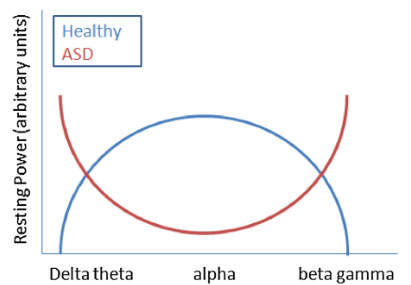
\includegraphics[width=0.5\textwidth]{assets/pics/ushaped.png}
    \caption{Ilustrasi \textit{U-shaped spectral profile} yang ditemukan pada pita frekuensi penderita ASD}
    \label{fig:ushape}
\end{figure}

Berdasarkan fitur yang diperoleh, proses klasifikasi dilakukan menggunakan algoritma \textit{machine learning} untuk membangun model prediksi. Berbagai metode seperti \textit{support vector machine} (SVM), \textit{k-nearest neighbor} (KNN), dan \textit{random forest} telah banyak digunakan dalam klasifikasi EEG dan menunjukkan performa yang baik dalam mengenali pola aktivitas neural yang kompleks \cite{ml_eeg_fnirs_review}. Meskipun pendekatan \textit{deep learning} berkembang pesat, metode \textit{machine learning} konvensional masih relevan terutama pada kondisi data terbatas dan kebutuhan interpretabilitas model \cite{ml_eeg_classification}.

\begin{figure}[H]
    \centering
    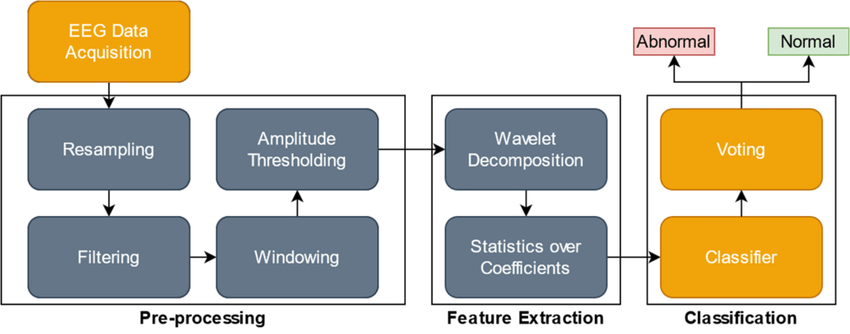
\includegraphics[width=0.8\textwidth]{assets/pics/general_pipeline.png}
  \caption{Ilustrasi umum pipeline klasifikasi ASD berbasis sinyal EEG}
    \label{fig:pipeline_asd_classification}
\end{figure}

Gambar \ref{fig:pipeline_asd_classification} menunjukkan proses klasifikasi berbasis sinyal EEG pada umumnya. Pipeline diawali akuisisi sinyal EEG, dilanjutkan dengan tahap \textit{preprocessing} untuk meningkatkan kualitas sinyal sebelum dianalisis lebih lanjut. Setelah itu, dilakukan proses ekstraksi fitur untuk memperoleh representasi informasi dari sinyal EEG yang relevan terhadap proses klasifikasi. Fitur yang diperoleh dari tahap ekstraksi kemudian digunakan sebagai masukan bagi model \textit{machine learning} untuk mempelajari pola-pola dalam sinyal EEG dan melakukan proses klasifikasi berupa prediksi terhadap kelas atau label yang telah ditentukan sesuai dengan tujuan penelitian. Secara umum, pipeline ini bertujuan mengubah sinyal EEG mentah menjadi representasi fitur yang lebih informatif dan terstruktur sehingga dapat diproses secara efektif oleh algoritma klasifikasi.

\subsection{Augmentasi Data EEG}
\label{Augmentasi Data EEG}
Performa model \textit{machine learning} sangat dipengaruhi oleh jumlah, kualitas, dan keragaman data \textit{training}. Pada analisis sinyal EEG, keterbatasan data menjadi tantangan karena proses akuisisi relatif mahal, memakan waktu, serta menghasilkan data dengan variabilitas tinggi antar individu maupun sesi \cite{cross_dataset_eeg}. Variabilitas tersebut dipengaruhi oleh perbedaan perangkat, konfigurasi kanal, kondisi eksperimen, aktivitas fisiologis, dan artefak non-neural, sehingga distribusi data EEG menjadi kompleks dan tidak konsisten antar dataset. Kondisi ini dapat menyebabkan model mengalami \textit{overfitting} dan memiliki kemampuan generalisasi yang rendah terhadap data baru.

Untuk mengatasi permasalahan tersebut, berbagai penelitian mengusulkan penggunaan teknik \textit{data augmentation} untuk meningkatkan jumlah dan variasi data \textit{training} tanpa memerlukan proses perekaman tambahan \cite{eeg_augmentation_review}. Secara umum, \textit{data augmentation} bertujuan menghasilkan sampel data baru yang tetap mempertahankan karakteristik utama data asli sehingga model dapat mempelajari representasi pola yang lebih stabil.

Pada sinyal \textit{time-series} seperti sinyal EEG, augmentasi konvensional umumnya dilakukan melalui manipulasi langsung terhadap sinyal dalam domain waktu maupun frekuensi \cite{traditional_timeseries_aug}. Pendekatan ini menghasilkan sampel baru dengan memodifikasi data asli menggunakan aturan transformasi tertentu tanpa mempelajari distribusi data secara eksplisit. Beberapa metode augmentasi yang umum digunakan pada data \textit{time-series} meliputi \textit{Flipping}, \textit{Down-sampling}, \textit{Adding Slope}, \textit{Amplitude Adjusted Fourier Transform (AAFT)}, \textit{Iterative Amplitude Adjusted Fourier Transform (IAAFT)}, \textit{Amplitude-Phase Perturbation (APP)}, dan \textit{Short-Time Fourier Transform (STFT)-based Augmentation}. Ilustrasi penerapan masing-masing metode ditunjukkan pada gambar \ref{fig:traditional_augmentation_example} dengan detail implementasi yang disajikan pada tabel \ref{tab:traditional_augmentation_methods}.

\begin{figure}[H]
    \centering
    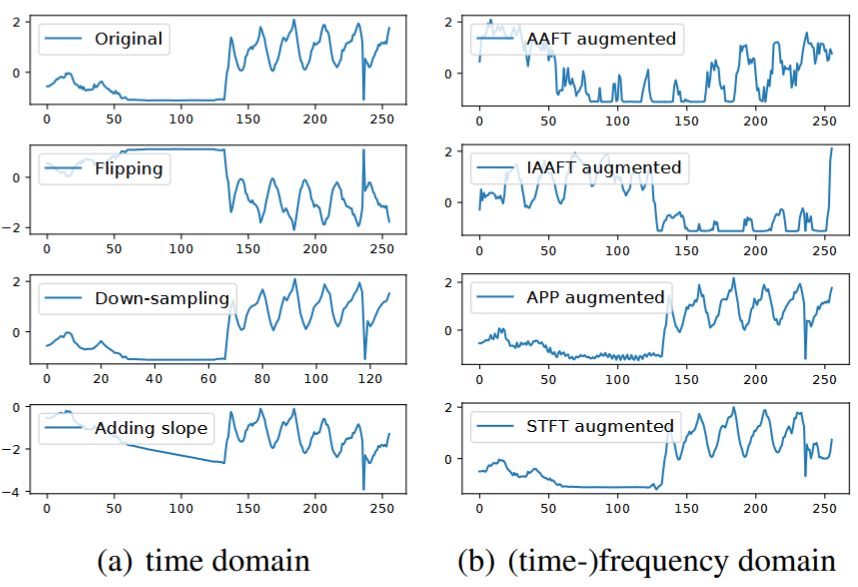
\includegraphics[width=\textwidth]{assets/pics/traditional_augmentation.png}
    \caption{Ilustrasi metode augmentasi pada data \textit{time-series}}
    \label{fig:traditional_augmentation_example}
\end{figure}

\begin{table}[H]
\centering
\footnotesize
\caption{Metode augmentasi pada data \textit{time-series}}
\label{tab:traditional_augmentation_methods}
\begin{tabular}{|c|c|p{6cm}|}
\hline
\textbf{Metode} & \textbf{Formula} & \textbf{Pengaruh terhadap Data} \\ \hline

\textit{Flipping} &
$x'(t) = -x(t)$ &
Membalik amplitudo sinyal terhadap sumbu horizontal sehingga pola temporal tetap terjaga tetapi orientasi sinyal berubah. \\ \hline

\textit{Down-sampling} &
$x'(t) = x(nt)$ &
Mengurangi jumlah sampel dengan faktor tertentu sehingga menghasilkan variasi resolusi temporal data. \\ \hline

\textit{Adding Slope} &
$x'(t) = x(t) + \alpha t$ &
Menambahkan tren linier pada sinyal untuk mensimulasikan perubahan gradual atau \textit{drift}. \\ \hline

\textit{AAFT} &
$x'(t)=\mathcal{F}^{-1}\!\left(|X(f)|e^{j\phi_r(f)}\right)$ &
Menghasilkan sinyal surrogate yang mempertahankan distribusi amplitudo dan spektrum daya secara aproksimatif. \\ \hline

\textit{IAAFT} &
$x'(t)=\mathrm{IAAFT}(x(t))$ &
Menghasilkan sinyal surrogate yang lebih akurat dalam mempertahankan distribusi amplitudo dan spektrum daya dibandingkan AAFT melalui proses iteratif. \\ \hline

\textit{APP} &
$X'(f)=A(f)e^{j(\phi(f)+\Delta\phi)}$ &
Menambahkan perturbasi pada amplitudo atau fase di domain frekuensi untuk menciptakan variasi sinyal yang realistis. \\ \hline

\textit{STFT-based Augmentation} &
$X'(m,\omega)=\mathrm{Aug}(X(m,\omega))$ &
Melakukan augmentasi pada representasi waktu-frekuensi sehingga karakteristik lokal sinyal dapat dimodifikasi tanpa mengubah struktur global secara signifikan. \\ \hline

\end{tabular}
\end{table}


Meskipun relatif sederhana dan mudah diterapkan, metode augmentasi konvensional memiliki keterbatasan dalam mempertahankan karakteristik kompleks sinyal EEG secara menyeluruh. Transformasi langsung terhadap sinyal berpotensi mengubah dependensi spasial maupun temporal yang penting dalam representasi aktivitas fisiologis. Selain itu, beberapa penelitian menunjukkan bahwa augmentasi sederhana tidak selalu meningkatkan performa model klasifikasi EEG secara konsisten. Oleh karena itu, penelitian lain mulai menggunakan pendekatan berbasis model generatif yang mampu mempelajari distribusi data untuk menghasilkan sampel sintetis yang lebih representatif terhadap karakteristik sinyal EEG.

\subsection{Model Generatif untuk Augmentasi Data}
\label{sec:model_generatif}

Model generatif merupakan pendekatan dalam \textit{machine learning} yang mempelajari distribusi dan pola suatu dataset untuk menghasilkan sampel data baru yang memiliki karakteristik serupa dengan data asli, berbeda dengan model diskriminatif yang digunakan pada proses klasifikasi atau prediksi label \cite{generative_models_survey}. Model generatif digunakan dalam berbagai aplikasi seperti sintesis gambar, rekonstruksi data (\textit{data reconstruction}), pemrosesan suara, hingga pembuatan data sintetis untuk kebutuhan \textit{training} model.

Data sintetis yang dihasilkan model generatif menjadi salah satu solusi terhadap berbagai permasalahan pada proses pengolahan data, seperti keterbatasan jumlah data, ketidakseimbangan kelas (\textit{class imbalance}), serta kendala privasi dan akuisisi data \cite{generative_models_survey}. Dalam konteks \textit{machine learning}, data sintetis yang dihasilkan oleh model generatif dapat digunakan sebagai bentuk \textit{data augmentation} untuk meningkatkan jumlah dan keragaman data \textit{training} tanpa memerlukan proses pengumpulan data baru secara langsung. Pendekatan ini memungkinkan model mempelajari representasi data yang lebih beragam sehingga dapat membantu meningkatkan kemampuan generalisasi model.

Berbagai arsitektur model generatif telah dikembangkan dalam penelitian \textit{deep learning}. Beberapa pendekatan yang umum digunakan meliputi \textit{Generative Adversarial Networks} (GAN), \textit{Variational Autoencoders} (VAE), serta model berbasis difusi (\textit{diffusion models}). Masing-masing pendekatan memiliki mekanisme pembelajaran dan karakteristik yang berbeda dalam menghasilkan data sintetis.

    \begin{table}[H]
    \centering
    \footnotesize
\caption{Perbandingan karakteristik, kelebihan, dan keterbatasan beberapa model generatif utama}
    \label{tab:generative_models}
    \begin{tabular}{|c|p{4cm}|p{5cm}|}
    \hline
    \textbf{Model} & \textbf{Karakteristik Utama} & \textbf{Kelebihan dan Keterbatasan} \\ \hline

    GAN &
    Menggunakan mekanisme kompetitif antara generator dan discriminator untuk menghasilkan data sintetis. &
    Mampu menghasilkan data yang realistis, namun proses \textit{training} cenderung tidak stabil dan rentan terhadap \textit{mode collapse}. \\ \hline

    VAE &
    Mempelajari distribusi laten probabilistik melalui arsitektur encoder-decoder. &
    Memiliki proses \textit{training} yang lebih stabil dan mampu menghasilkan representasi laten yang terstruktur, namun kualitas data sintetis dapat lebih halus dibanding GAN. \\ \hline

    Diffusion Model &
    Menghasilkan data melalui proses denoising bertahap dari distribusi acak. &
    Mampu menghasilkan kualitas data yang tinggi, namun memerlukan kompleksitas komputasi dan waktu \textit{training} yang lebih besar. \\ \hline

    \end{tabular}
    \end{table}

Dalam analisis sinyal EEG, model generatif digunakan untuk menghasilkan data sintetis yang mengikuti distribusi statistik data asli. Pendekatan ini memungkinkan model mempelajari struktur laten dari sinyal EEG sehingga data sintetis yang dihasilkan dapat mempertahankan karakteristik temporal maupun spasial yang penting dalam proses klasifikasi. Beberapa penelitian menunjukkan bahwa penggunaan data sintetis dari model generatif dapat membantu meningkatkan performa dan kemampuan generalisasi model klasifikasi EEG, terutama pada kondisi jumlah data \textit{training} yang terbatas \cite{gan_eeg_emotion}.

Salah satu model generatif yang banyak digunakan dalam augmentasi data EEG adalah \textit{Variational Autoencoder} (VAE). Dibandingkan GAN, VAE memiliki proses \textit{training} yang lebih stabil dan tidak bergantung pada mekanisme adversarial yang rentan terhadap \textit{mode collapse}. Selain itu, dibandingkan \textit{diffusion model}, VAE umumnya memerlukan kompleksitas komputasi dan jumlah data \textit{training} yang lebih rendah. Karakteristik tersebut menjadikan VAE lebih sesuai untuk penelitian ini yang menggunakan dataset EEG dengan jumlah data terbatas\cite{eeg_augmentation_review}.   


\subsection{Variational Auto Encoder}
\label{Variational AutoEncoder}
\textit{Variational Autoencoder} (VAE) merupakan salah satu model generatif berbasis \textit{deep learning} yang digunakan untuk mempelajari representasi laten dari suatu dataset dan menghasilkan sampel data baru dengan karakteristik yang serupa dengan data asli. Berbeda dengan \textit{autoencoder} konvensional yang berfokus pada proses kompresi dan rekonstruksi data, VAE memodelkan representasi laten sebagai distribusi probabilistik sehingga memungkinkan proses generasi data baru melalui ruang laten (\textit{latent space}) yang dipelajari oleh model \cite{cvae_gan_eeg}.

\begin{figure}[H]
    \centering
    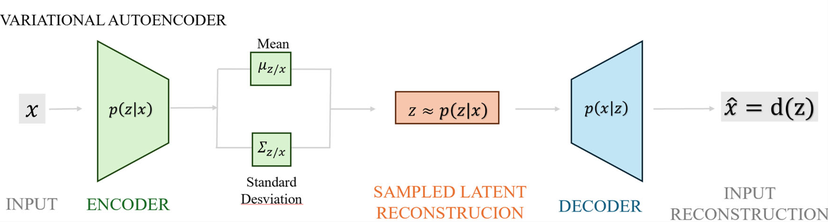
\includegraphics[width=0.8\textwidth]{assets/pics/vae-architecture.png}
    \caption{Arsitektur umum \textit{Variational Autoencoder} (VAE)}
    \label{fig:vae_architecture}
\end{figure}


Arsitektur VAE terdiri atas dua komponen utama, yaitu \textit{encoder} dan \textit{decoder}, seperti yang diilustrasikan pada Gambar \ref{fig:vae_architecture}. \textit{Encoder} bertugas memetakan data input ke representasi laten berdimensi lebih rendah dalam bentuk parameter distribusi probabilistik, yaitu nilai rata-rata ($\mu$) dan variansi ($\sigma$). Representasi laten tersebut kemudian digunakan oleh \textit{decoder} untuk merekonstruksi kembali data sehingga menghasilkan output yang memiliki karakteristik serupa dengan data asli.

Proses \textit{training} VAE dilakukan menggunakan fungsi objektif \textit{Evidence Lower Bound} (ELBO), yang terdiri atas dua komponen utama, yaitu \textit{reconstruction loss} dan \textit{Kullback--Leibler Divergence} (KL Divergence). \textit{Reconstruction loss} digunakan untuk mengukur kualitas hasil rekonstruksi data, sedangkan KL Divergence berfungsi menjaga distribusi laten agar tetap mendekati distribusi normal standar. Secara matematis, fungsi objektif VAE dirumuskan sebagaimana pada persamaan \ref{eq:elbo}:
\begin{equation}
\mathcal{L}(\theta, \phi; x) =
\mathbb{E}_{q_{\phi}(z|x)}[\log p_{\theta}(x|z)] -
D_{KL}(q_{\phi}(z|x) \parallel p(z))
\label{eq:elbo}
\end{equation}
di mana $q_{\phi}(z|x)$ merepresentasikan distribusi laten yang dihasilkan oleh \textit{encoder}, $p_{\theta}(x|z)$ merepresentasikan proses rekonstruksi oleh \textit{decoder}, dan $p(z)$ merupakan distribusi prior pada ruang laten. Komponen pertama pada persamaan tersebut merepresentasikan kualitas rekonstruksi data, sedangkan komponen kedua berfungsi sebagai regularisasi untuk menjaga struktur distribusi laten \cite{vae_original}.

Proses \textit{sampling} pada ruang laten tidak dapat dilakukan secara langsung dalam proses \textit{training} menggunakan metode \textit{backpropagation}. Oleh karena itu, VAE menggunakan teknik yang dikenal sebagai \textit{reparameterization trick}. Melalui teknik ini, variabel laten $z$ dinyatakan sebagaimana yang terlihat pada persamaan \ref{eqz}. 
\begin{equation}
z = \mu + \sigma \cdot \epsilon
\label{eqz}
\end{equation}

di mana $\epsilon$ merupakan variabel acak yang diambil dari distribusi normal standar $\mathcal{N}(0,1)$. Dengan pendekatan ini, proses \textit{sampling} dapat ditransformasikan menjadi operasi deterministik yang memungkinkan gradien tetap dapat dihitung selama proses \textit{training} neural network \cite{vae_original}.


\subsection{Metode Evaluasi Data Sintetis Sinyal EEG}

Evaluasi kualitas data sintetis diperlukan untuk menilai sejauh mana sinyal EEG yang dihasilkan model generatif mampu mempertahankan karakteristik data asli. Dalam penelitian referensi \cite{eeg_gan}, evaluasi dilakukan menggunakan beberapa metrik kuantitatif yang umum digunakan pada model generatif, yaitu, \textit{Frechet Inception Distance} (FID), \textit{Euclidean Distance} (ED), dan \textit{Sliced Wasserstein Distance} (SWD). Definisi, formulasi matematis, serta aspek kualitas data yang dievaluasi oleh masing-masing metrik dirangkum dalam tabel \ref{tab:evaluation_metrics}.

\begin{table}[H]
\centering
\footnotesize
\caption{Metrik evaluasi data sintetis EEG}
\label{tab:evaluation_metrics}
\renewcommand{\arraystretch}{1.5}
\resizebox{\textwidth}{!}{
\begin{tabular}{|c|p{6cm}|p{5cm}|}
\hline
\textbf{Metrik} & \textbf{Formula} & \textbf{Aspek yang Dievaluasi} \\ \hline

\textit{Frechet Inception Distance} (FID) &
$\displaystyle
\|\mu_r-\mu_g\|^2 +
Tr(\Sigma_r+\Sigma_g
-2(\Sigma_r\Sigma_g)^{1/2})
$
&
Mengukur kesamaan distribusi fitur antara data asli dan sintetis. \\ \hline

\textit{Euclidean Distance} (ED) &
$\displaystyle
d(x,y)=
\sqrt{
\sum_{i=1}^{n}(x_i-y_i)^2
}
$
&
Mengukur kemiripan langsung antar sampel data asli dan sintetis. \\ \hline

\textit{Sliced Wasserstein Distance} (SWD) &
$\displaystyle
SWD(P,Q)=
\int_{\theta}
W_1(P_{\theta},Q_{\theta})
\, d\theta
$
&
Mengukur kesamaan distribusi global melalui proyeksi satu dimensi. \\ \hline

\end{tabular}
}
\end{table}

Penelitian referensi \cite{eeg_gan} menunjukkan bahwa tidak terdapat satu metrik yang mampu merepresentasikan seluruh karakteristik kualitas sinyal EEG sintetis secara menyeluruh. Pada penelitian tersebut, nilai FID yang rendah tidak selalu menunjukkan kesamaan karakteristik spasial dan spektral terhadap data asli, sedangkan SWD dinilai lebih mampu merepresentasikan distribusi sinyal yang natural. Oleh karena itu, penggunaan beberapa metrik evaluasi secara bersamaan diperlukan untuk memperoleh penilaian kualitas data sintetis yang lebih komprehensif.

\section{Penelitian Terdahulu}
\label{Penelitian Terdahulu}

Berbagai penelitian telah mengusulkan pendekatan \textit{machine learning} untuk klasifikasi \textit{Autism Spectrum Disorder} (ASD) berbasis sinyal EEG dengan memanfaatkan karakteristik aktivitas neural sebagai fitur klasifikasi. Selain itu, beberapa penelitian juga menerapkan teknik augmentasi data untuk mengatasi keterbatasan jumlah data \textit{training} dan meningkatkan performa model klasifikasi.

Tinjauan terhadap penelitian terdahulu diperlukan untuk memahami perkembangan metode klasifikasi EEG, pendekatan augmentasi data yang telah digunakan, serta keterbatasan yang masih menjadi tantangan dalam pengembangan sistem klasifikasi ASD berbasis EEG.

\subsection{Klasifikasi ASD Berbasis EEG Menggunakan Kombinasi mRMR dan XGBoost}
\label{Klasifikasi ASD Berbasis EEG Menggunakan mRMR dan XGBoost}

Pada penelitian rujukan \cite{paper_ref}, klasifikasi \textit{Autism Spectrum Disorder} (ASD) dilakukan menggunakan sinyal EEG dengan memanfaatkan seleksi fitur dan algoritma \textit{machine learning}. Penelitian berfokus pada penggunaan fitur domain frekuensi untuk merepresentasikan karakteristik aktivitas neural yang berkaitan dengan ASD serta meningkatkan performa klasifikasi melalui pemilihan fitur yang optimal.

Penelitian menggunakan metode \textit{minimum Redundancy Maximum Relevance} (mRMR) untuk memilih fitur yang paling relevan dan memiliki redundansi minimum antar fitur. Sebelum proses seleksi fitur, sinyal EEG melalui tahap \textit{preprocessing} seperti segmentasi, \textit{filtering}, dan dekomposisi pita frekuensi. Fitur hasil seleksi kemudian digunakan sebagai masukan bagi model klasifikasi berbasis \textit{ensemble}, yaitu XGBoost. Performa metode tersebut dibandingkan dengan model \textit{Deep Neural Network} (DNN) sebagai metode \textit{baseline}, sehingga peningkatan performa yang diperoleh dievaluasi berdasarkan hasil perbandingan terhadap model DNN.

Hasil penelitian menunjukkan bahwa kombinasi mRMR dan XGBoost mampu memberikan performa klasifikasi yang baik dalam membedakan individu ASD dan non-ASD. Penggunaan mRMR membantu meningkatkan kualitas fitur, sementara XGBoost memberikan kemampuan klasifikasi yang robust terhadap kompleksitas data EEG. Namun, penelitian juga menunjukkan bahwa pendekatan tersebut memiliki waktu komputasi yang lebih tinggi dibandingkan model dasar yang digunakan sebagai pembanding. Selain itu, penelitian masih dilakukan pada jumlah dataset yang relatif terbatas, sehingga kemampuan generalisasi model masih menjadi tantangan dalam pengembangan sistem klasifikasi EEG berbasis ASD. 

\subsection{Metode Augmentasi Data pada Sinyal EEG Menggunakan Variational Autoencoder}
\label{Augmentasi Data pada Sinyal EEG Menggunakan Variational Autoencoder}

Pada penelitian rujukan \cite{gan_eeg_emotion}, digunakan pendekatan augmentasi data berbasis \textit{Variational Autoencoder} (VAE) untuk menghasilkan sinyal EEG sintetis pada tugas klasifikasi \textit{motor imagery}. Penelitian memanfaatkan BCI Competition IV Dataset 2a yang terdiri dari data EEG 22 kanal dari 9 subjek. Data EEG direpresentasikan dalam bentuk matriks dua dimensi untuk menyesuaikan penggunaan arsitektur berbasis \textit{2D Convolutional Neural Network} (2D CNN).

Model VAE terdiri dari komponen \textit{encoder} dan \textit{decoder} yang digunakan untuk mempelajari representasi laten dari sinyal EEG dan merekonstruksi kembali data sintetis yang menyerupai data asli. Untuk evaluasi klasifikasi, penelitian menggunakan arsitektur EEGNet dan membandingkan performa model yang dilatih menggunakan data asli dengan model yang dilatih menggunakan data hasil augmentasi.

Hasil penelitian menunjukkan bahwa penggunaan data sintetis dari VAE mampu meningkatkan performa klasifikasi secara signifikan, di mana akurasi meningkat dari 0.73 menjadi 0.88. Peningkatan juga terlihat pada metrik \textit{precision}, \textit{recall}, dan \textit{f1-score}, yang menunjukkan bahwa data sintetis mampu memperkaya variasi data \textit{training}.

Namun, penelitian tersebut masih berfokus pada representasi sinyal EEG dalam domain waktu dan belum mempertimbangkan karakteristik domain frekuensi secara menyeluruh. Padahal, analisis domain frekuensi memiliki peran penting dalam identifikasi pola neurofisiologis pada EEG, termasuk pada studi ASD, karena informasi aktivitas neural banyak direpresentasikan melalui distribusi daya pada pita frekuensi tertentu.

\subsection{Dataset EEG yang Digunakan dalam Penelitian}
\label{Dataset EEG yang Digunakan}

Dataset yang digunakan dalam penelitian ini berupa sinyal \textit{electroencephalogram} (EEG) dari studi rujukan \cite{eeg_dataset_asd}, yang terdiri dari data subjek dengan dan tanpa diagnosis \textit{Autism Spectrum Disorder} (ASD). Dataset ini digunakan karena mampu merepresentasikan karakteristik aktivitas neural yang berkaitan dengan ASD sehingga relevan untuk pengembangan model klasifikasi berbasis \textit{machine learning}.

Data EEG dikumpulkan dari sepuluh partisipan yang terdiri dari lima anak dengan ASD berusia 6--10 tahun dan lima subjek kontrol sehat. Akuisisi dilakukan menggunakan perangkat \textit{OpenBCI Cyton Biosensing Board} dengan 16 kanal EEG berdasarkan sistem \textit{International 10--20 System}. Proses perekaman dilakukan tanpa stimulus eksternal dengan upaya meminimalkan distraksi partisipan untuk menjaga kualitas sinyal EEG yang diperoleh.

Setelah akuisisi, sinyal EEG melalui tahap \textit{preprocessing} menggunakan metode seperti \textit{Butterworth filtering}, \textit{Discrete Wavelet Transform} (DWT), dan \textit{Independent Component Analysis} (ICA) untuk mengurangi artefak dan meningkatkan kualitas sinyal \cite{paper_ref}. Selanjutnya, sinyal diproses melalui segmentasi dan dekomposisi ke dalam pita frekuensi utama seperti delta, theta, alpha, beta, dan gamma untuk proses ekstraksi fitur dan klasifikasi.

Meskipun dataset ini relevan untuk analisis ASD berbasis EEG, jumlah partisipan yang relatif kecil menjadi salah satu keterbatasan penelitian. Dataset hanya mencakup data dari sepuluh subjek sehingga berpotensi membatasi kemampuan generalisasi model serta meningkatkan risiko \textit{overfitting}, khususnya pada model \textit{machine learning} yang memerlukan jumlah data \textit{training} yang lebih besar.

\section{Fokus pada Celah Penelitian}
\label{Fokus pada Celah Penelitian}

Berdasarkan tinjauan pustaka yang telah dilakukan, terdapat celah penelitian dalam pemanfaatan teknik augmentasi data berbasis \textit{Variational Autoencoder} (VAE) untuk analisis sinyal EEG. Beberapa penelitian sebelumnya telah menerapkan VAE untuk menghasilkan data EEG sintetis, khususnya dalam konteks tugas klasifikasi berbasis \textit{motor imagery} menggunakan arsitektur seperti \textit{2D Convolutional Neural Network} (CNN). Pendekatan tersebut menunjukkan bahwa data sintetis mampu meningkatkan performa model klasifikasi dengan memperkaya variasi data \textit{training}. Meskipun demikian, fokus penelitian masih terbatas pada representasi sinyal dalam domain waktu atau spasial, tanpa mengeksplorasi secara mendalam karakteristik sinyal dalam domain frekuensi.

Di sisi lain, analisis berbasis domain frekuensi memiliki peran penting dalam studi EEG, terutama dalam mengidentifikasi pola osilasi neural yang berkaitan dengan kondisi neurologis seperti \textit{Autism Spectrum Disorder} (ASD). Pemanfaatan data sintetis berbasis VAE pada representasi fitur frekuensi masih relatif terbatas, dan belum banyak dilakukan pengkajian terkait pengaruh augmentasi sinyal EEG terhadap kualitas fitur dan performa model klasifikasi berbasis \textit{machine learning} konvensional.

Oleh karena itu, penelitian ini mengusulkan pendekatan yang mengintegrasikan teknik augmentasi data berbasis VAE dengan ekstraksi fitur domain frekuensi, serta memanfaatkan metode seleksi fitur \textit{minimum Redundancy Maximum Relevance} (mRMR) dan algoritma klasifikasi \textit{XGBoost}. Pendekatan ini bertujuan untuk mengeksplorasi bagaimana data sintetis yang dihasilkan pada domain frekuensi dapat meningkatkan kualitas representasi fitur serta performa klasifikasi ASD. Dengan mengisi celah ini, diharapkan penelitian ini dapat memberikan kontribusi dalam pengembangan metode klasifikasi EEG yang lebih robust dan akurat, khususnya pada kondisi dataset yang terbatas.



%
% Daftar Pustaka
%\input{pustaka}

% Alternatif manajemen daftar pustaka dengan \bibliography
\bibliographystyle{IEEEtran}
\bibliography{pustaka}

%
% Lampiran 
%
% \begin{appendix}
% 	\input{_internals/markLampiran}
% 	\setcounter{page}{2}\textbf{}
% 	\input{src/99-back_matter/lampiran}
% \end{appendix}

\end{document}